\chapter{Implementación}

Para la implementación de la solución utilizaremos una arquitectura cliente-servidor\cite{client-server}, la cual nos
permite tener los datos centralizados en una aplicación servidor. La aplicación cliente realizará peticiones al
servidor, para que este le provea de los datos que necesite en cada momento.\\

\section{Servidor}
En el lado del servidor o \textit{back-end} se encuentra la mayor parte de la lógica de la aplicación, dedicándose el
lado del cliente a simplemente mostrarla en una interfaz cómoda para el usuario.\\

Se ha implementado un servidor que provee a los clientes de un listado de series y sus temporadas, así como de la
posibilidad de crear reseñas de las mismas o obtener las reseñas de otros usuarios.

\subsection{Lenguaje de programación}
El lenguaje de programación seleccionado para el servidor es \textit{Python}\cite{python}, ya que es un lenguaje de
programación que nos provee de una buena experiencia de desarrollo al ser un lenguaje menos estricto y cuenta con muchas
librerías útiles y una enorme comunidad a sus espaldas.\\

Uno de sus puntos débiles, es que al ser un lenguaje no tipado, es más propenso a errores de sintaxis, pero desde la
versión 3.5, cuenta con una forma de tipar el código, de forma que, aunque el intérprete de \textit{Python} no detecte
este tipado, puede ser utilizado por herramientas de los \textit{IDEs} y \textit{linters} para la detección precoz
errores.\\

Otro de los motivos que me han llevado a decantarme por este lenguaje son sus librerías científicas y de procesamiento
de datos. Con ellas, en un futuro podríamos incluir en la aplicación alguna herramienta para obtener estadísticas y
realizar predicciones sobre nuestros datos. Algo muy útil para un cliente que quiera usar los datos de la aplicación
para saber qué tipo de series interesan a cierto tipo de público, por ejemplo.\\

Como gestor de paquetes y dependencias, utilizo \textit{poetry}\cite{poetry}, que nos permite gestionar las dependencias
del proyecto de forma muy sencilla y similar a \textit{NPM}\cite{npm}.

\subsection{Framework}
El framework utilizado para el servidor es \textit{Flask}\cite{flask}, un framework de Python que nos permite una 
\textit{REST API}\cite{rest} minimalista, flexible y fácil de usar.

\subsection{Operaciones}
Recopilación y breve descripción de las peticiones que atiende el servidor.

\subsubsection{Series}
El servidor provee de una lista de series o de los detalles de una serie en particular o alguna de sus temporadas a
través de su identificador. Sin embargo, la base de datos no incluye la información de estas series, si no que se
obtienen a través de una API externa.\\

La API utilizada es \href{https://www.themoviedb.org}{\textit{TheMovieDB}}, una API abierta que provee de datos sobre
series y películas. En este caso, haremos uso de las series. Gracias al diseño de nuestra aplicación, podríamos cambiar
de API en cualquier momento, sin que suponga mucho tiempo de desarrollo.

\subsubsection{Usuarios}
Cualquiera podrá crear un usuario, siempre y cuando el email introducido no esté en uso.\\

Los usuarios podrán loguearse con su cuenta, lo que generará un token de acceso que deberá ser enviado en las cabeceras
del resto de peticiones, para identificar qué usuario está realizando la petición. Las operaciones sobre las series no
requieren de autenticación, pero sí las operaciones sobre las reseñas.\\

Para asegurarnos que el usuario está logueado, utilizamos un \textit{decorador} de la librería
\textit{Flask-JWT-Extended}\cite{jwt} que comprueba que el token enviado en las cabeceras de la petición es válido. Si
no lo es, se devuelve un error 401, o de desautorización.\\

\subsubsection{Reseñas}
Los usuarios logueados podrán crear reseñas de las series. Usando el token \textit{JWT} del que hablamos en la sección
anterior, podemos obtener el identificador del usuario que está realizando la petición y añadirlo a los datos de la
reseña.\\ 

\subsection{Test}
Como ya hablamos en la \hyperref[chap:metodología]{metodología}, necesitamos que el código cumpla con unos requisitos
mínimos de calidad a través de \textit{tests}.\\

Para el servidor, se han implementado tests unitarios con la librería \textit{pytest}\cite{pytest}, que comprueban que
los métodos de los modelos de la aplicación funcionan correctamente.
\begin{figure}[H]
\centering	
    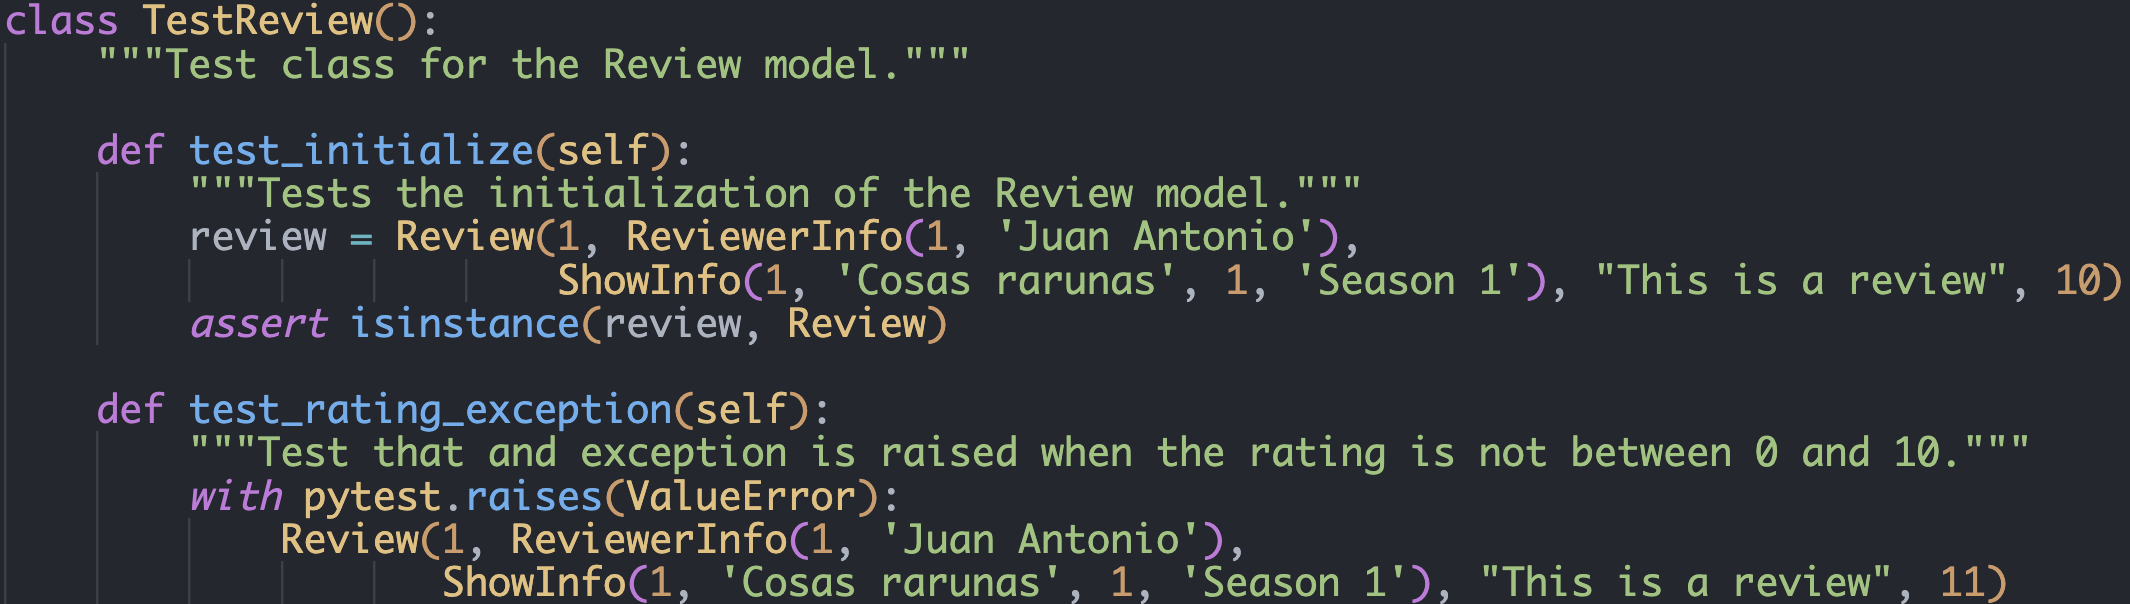
\includegraphics[scale=0.25]{img/pytest.png}
\caption{ Test unitario de la clase Show en Python }\label{fig:pytest}
\end{figure}

\subsection{Base de datos}
El número de reseñas irá en aumento con el tiempo y con el número de usuarios de la aplicación, por lo que necesito una
base de datos que sea fácilmente escalable. Por ello, \textit{MongoDB}\cite{mongodb} es una muy buena opción, gracias a
\textit{MongoAtlas}\cite{mongoatlas}, una herramienta \textit{DataBase as a Service}\cite{dbaas} que nos permite escalar
la base de datos verticalmente, aumentando el poder de procesamiento de nuestro cluster, u horizontalmente, añadiendo
más nodos para compartir la carga.\\

Además, guarda los datos en formato \textit{JSON}\cite{json}, lo que nos permite acceder a ellos de forma muy sencilla y
fácilmente interpretable por cualquier lenguaje de programación moderno.

\subsection{Configuración}

Las variables de configuración se encuentran en los ficheros del directorio \textit{config} y se definen mediante las
variables de entorno, incluyendo opciones por defecto en la mayoría. En el entorno de desarrollo, uso \textit{dotenv}
para cargar las variables de entorno desde un fichero de configuración \textit{.env}.
\begin{figure}[H]
\centering	
    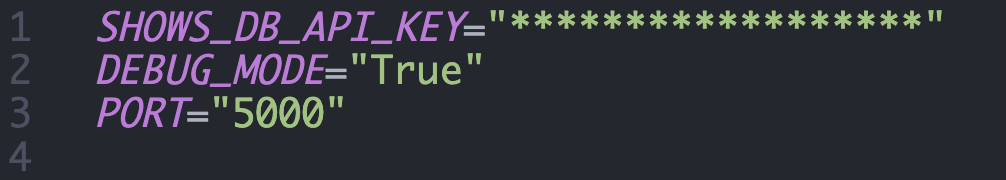
\includegraphics[scale=0.525]{img/dotenv.png}
\caption{ Fichero de configuración con las variables de entorno del servidor }\label{fig:dotenv}
\end{figure}

\section{Cliente}
El cliente o \textit{back-end} es la parte de la aplicación que se ejecuta en el dispositivo del usuario. En nuestro
caso, la mayor parte de la lógica se encuentra en el lado del servidor y el cliente se encarga de mostrar la información
y dar acceso a las peticiones del servidor de una forma amigable para el usuario.\\

\subsection{Elección de la tecnología}
Con el paso del tiempo, cada vez más frameworks y librerías se han ido desarrollando para la creación de aplicaciones
cliente, por lo que hay una gran variedad de tecnologías a nuestra disposición.\\

\subsubsection{Aplicación web vs aplicación móvil}
Es cierto que las aplicaciones móviles están ganando cada vez más popularidad, ya que con la afluencia de dispositivos
inteligentes como teléfonos, tablets, televisores e incluso frigoríficos, es más fácil acceder a la información desde
cualquier parte.\\

No por ello, debemos descartar las aplicaciones web. En este caso, una aplicación web es una solución sólida al
problema, al ser más cómodo para los usuarios escribir sus reseñas con su teclado y ratón, y no con su pantalla
táctil.\\

\subsubsection{Frameworks}
Los tres grandes framework para aplicaciones web son: \textit{Angular}\cite{angular}, \textit{React}\cite{react} y
\textit{Vue}\cite{vue}.\\

\noindent \textbf{Vue}\\ \\
\indent \textit{Vue} es un framework muy ligero, que se basa en componentes, lo que lo hace muy fácil de aprender y de usar.
Además, permite usar expansiones de terceros para añadir componentes o funcionalidades hechas por la comunidad. Sin
embargo, utiliza \textit{JavaScript}\cite{javascript} como lenguaje de programación, por lo que no es la opción más
deseable frente a los otros dos.\\

\noindent \textbf{React}\\ \\
\indent \textit{React} está basado en \textit{JavaScript} y utiliza \textit{JSX}\cite{jsx} para definir los componentes, aunque
también se puede usar \textit{TypeScript}\cite{typescript}, un lenguaje tipado que se transpila a \textit{JavaScript},
lo que nos permite la detección rápida de errores. Es un framework muy popular y con una gran comunidad detrás, lo que
lo convierte en una buena opción.\\

\noindent \textbf{Angular}\\ \\
\indent Finalmente, el framework que he elegido es \textit{Angular}. Aunque esté perdiendo popularidad, sigue
siendo una gran opción para el desarrollo de aplicaciones web. Trabaja nativamente con \textit{TypeScript}, por lo que
fácilmente podremos disfrutar de las ventajas de un lenguaje tipado.\\

\textit{Angular} es un framework diseñado y mantenido por \textit{Google} que nos ofrece un código bien estructurado
basado en componentes y servicios, que nos permite desarrollar con una arquitectura limpia y mantenible. Además, nos
permite usar \textit{Angular Material}\cite{angularmaterial}, un conjunto de componentes de \textit{Angular} que nos
permite crear interfaces de usuario modernas de forma rápida y sencilla y también cuenta con \textit{Ionic}\cite{ionic},
un framework para crear aplicaciones híbridas para móviles y web si en algún momento decidiésemos dar el salto a las
aplicaciones móviles.\\


